\documentclass[a4paper,10pt]{article}
\usepackage[utf8]{inputenc} % load international character 
\usepackage{graphicx}
\usepackage{url}

%opening -- comments
\title{Workshop}
\author{AAA   
					\and BBBB}

\begin{document}

	%Update title which is declare in opening section
	\maketitle
	
	%Update table content automatically
	\tableofcontents

\section[other name]{First Section}
\section{Second Section}
	\subsection{sub section 1}
		\paragraph{first paragraph}
			some text  -- testing %comments
			
			% --  $ for math mode		
			% -- { } adding space at the end 
			
			some text \^{ } testing.ååååå
			
			$\sim$
			
			``quote'' \rq\rq
			
			
			\pagebreak % breack a page with stretching
			\newpage %new page command
			
			\lq\lq quote''
			~  % unbreakable line
			% \LaTeX
			
			% new paragraph \\
			% \newline % newline with not stretching
			% \breakline % new line wih stretching

			
			%
			{
			\rmfamily
			\bfseries
			% \centering
			% \tiny
			You are the most welcome
			}
			
			% Can write separate chapters them include in other
			% chapter_1.tex
			% subfolder/chapter_2.tex
			% \input{chapter_1}
			% \input{subfolder/chapter_2.tex}
			
			% Enumerate
			\begin{enumerate}
				\item[a] A
				\item[2] B
				\item D
				\item[c] C
				\begin{enumerate}
					\item ADASD
				\end{enumerate}
				\begin{itemize}
					\item [+]ajfdlajsldf
				\end{itemize}
			\end{enumerate}
			
			% Math equation
			$$1 + 1 = 2 $$
			\begin{equation}
				1 + 1 = 2
			\end{equation}
			
			% Table or {table}
			\begin{table}
			\centering
				\begin{tabular}{|c|l|p{0.5\textwidth}|}
					1 & 2 & long lieth\\
					A & B & laongaoglj\\ \hline
					D & E & F
				\end{tabular}
				\caption{some caption}
			\end{table}

	
			% Adding picture
			\begin{figure}[h!] %here top bottom   -[h!]  here
				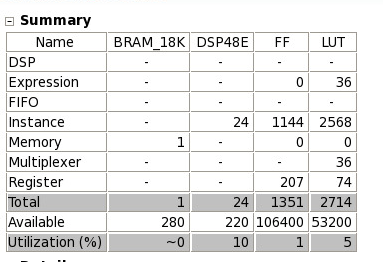
\includegraphics[scale=1]{img.jpg}
			\caption{logo}
			\label{logo}}
			\end{figure}
			
			\vfill
			footnote\footnote{Text of footnote}			
			\\
			another footnote\footnote{\url{google.com}}. As can be seen in figure ~/ref{logo}
			
			e. g.\ duck			
			
			\begin{quotation}
				The best
			\end{quotation}
\end{document}